\documentclass[bachelor]{XJTUthesis}

\begin{document}

\firstpage{西安交通大学}{\LaTeX 毕业设计模板}{电气学院}{电气工程}{电气613}{谢晋安}{0000000000}{谢晋安}{西安交通大学}

\tableofcontents
\thispagestyle{empty}
\setcounter{page}{0}
\newpage

\begin{abstract}
这是一个模板。
\end{abstract}
\keywords{\LaTeX;XJTU}
\newpage
\begin{eabstract}
This is a template.
\end{eabstract}
\ekeywords{\LaTeX;XJTU}

\chapter{图表}
图\ref{xiaohui:ref}和\ref{xiaohui:blue}是交大的校徽。
\begin{figure}[htbp]
  \centering
  
\includegraphics[width=0.3\textwidth]{figures//a3_1jdxhred.png}
  \caption{校徽}\label{xiaohui:red}
\end{figure}

图\ref{xiaohui}是交大的校徽。
\begin{figure}[htbp]
  \centering
  
\includegraphics[width=0.3\textwidth]{figures//a3_2jdxhblue.png}
  \caption{校徽}\label{xiaohui:blue}
\end{figure}

图\ref{xiaobiao}是交大的校标
\begin{figure}[htbp]
  \centering
  
\includegraphics[width=1\textwidth]{figures//a4_2xbred.png}
  \caption{校标}\label{xiaobiao}
\end{figure}

图\ref{xiaoxun}是交大的校训
\begin{figure}[htbp]
  \centering
  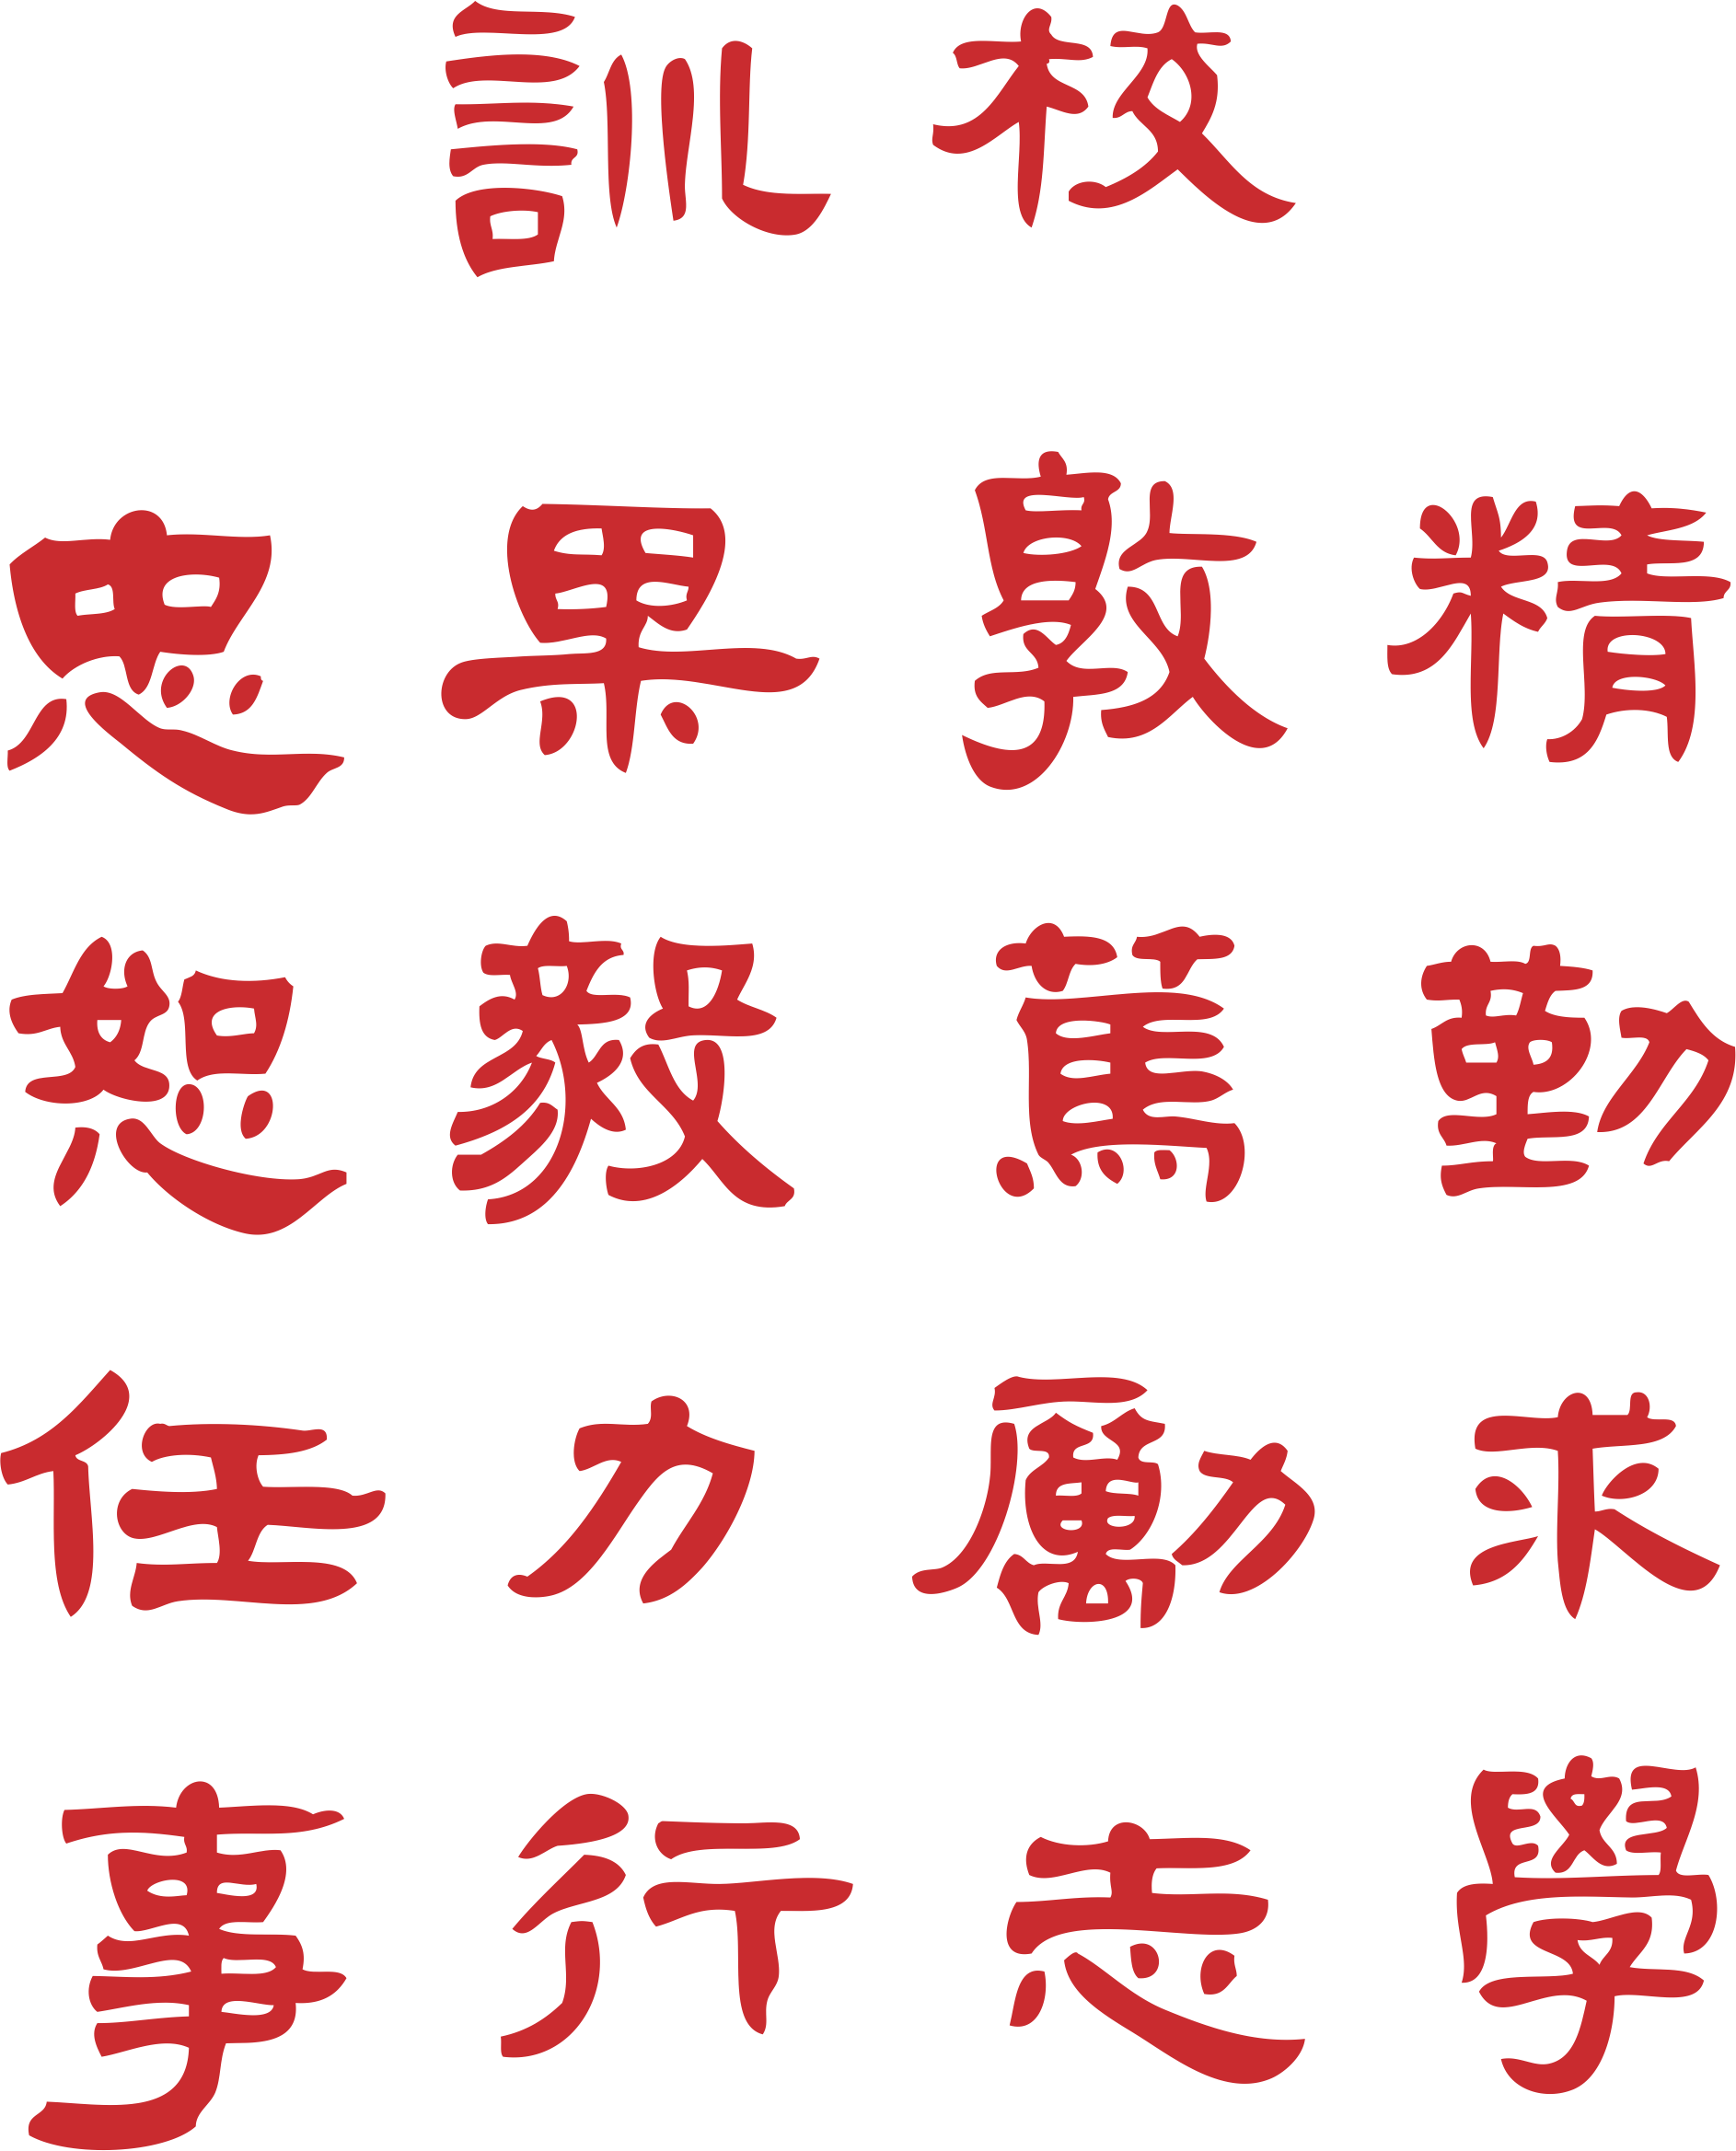
\includegraphics[width=0.5\textwidth]{figures//a5_2xxys2.png}
  \caption{校训}\label{xiaoxun}
\end{figure}

表\ref{fuhao}是符号说明
\begin{table}[htbp]
  \centering
\begin{tabular}{|c|c|}
  \hline
  
  \makecell{符号}&\makecell{说明}\\ %makecell用于生成表头
  \hline
  $a_t$ & 参数在t时刻的值 \\
  \hline
  $\rho$ & 相关系数 \\
  \hline
  $\boldsymbol{\omega}$ & 超平面方向向量 \\
  \hline
  $b$ & 超平面偏置量 \\
  \hline
\end{tabular}
  \caption{符号说明}\label{fuhao}
\end{table}

\chapter{图表2}
图\ref{xioabioa:shu}是竖版校标
\begin{figure}[htbp]
  \centering
  
\includegraphics[width=0.5\textwidth]{figures//a4_7sbzh.png}
  \caption{校标}\label{xioabioa:shu}
\end{figure}

\chapter{TIKZ}

\chapter{一些环境}

\chapter{杂项}

\end{document} 